%! Author = kubec
%! Date = 14.03.2024

% Preamble
\documentclass[11pt]{article}

% Packages
\usepackage{amsmath}
\usepackage{mathtools}
\usepackage{ragged2e}
\usepackage [utf8]{inputenc}
\usepackage{blindtext}
\usepackage{wrapfig}
\usepackage{xcolor}
\usepackage {polski}
\usepackage{multicol}
\usepackage[a4paper, total={5.7in, 8in}]{geometry}
\usepackage{graphicx}
\usepackage{amstex}
\usepackage{csvsimple}
\usepackage{changepage}
\usepackage{enumitem}
\usepackage[english]{babel}
\usepackage{biblatex}
\usepackage{caption}
\usepackage{indentfirst}

% Document
\begin{document}
%    Nagłówek
    \begin{flushleft}
        Filip Krauz-Damski 267 681 \hfill Data wykonania ćwiczenia:\\
        Filip Kubecki 272 655 \hfill 11 marca 2024r\\
        \hfill Data sporządzenia sprawozdania:\\
        Grupa: Pon 13:15 \hfill 16 marca 2024r\\
    \end{flushleft}
    \begin{center}
        \Large\textbf{Ćwiczenie 1.}\\
        \textbf{Podstawowe narzędzia pomiarowe w elektronice}
    \end{center}
    \vspace{1cm}

%    Treść
    \section{Spis przyrządów}
    \par{
        Do wykonania ćwiczenia wykorzystano:
        \begin{itemize}
            \setlength\itemsep{0em}
            \item[-] Przenośny multimetr analogowy AX-7003
            \item[-] Przenośny multimetr cyfrowy AX-MS8221A
            \item[-] Multimetr cyfrowy Agilent 34401A
            \item[-] Zasilacz laboratoryjny symetryczny Zhaoxin RXN-305DII
        \end{itemize}
    }
    \section{Przebieg i cel ćwiczenia}
    \par{
        Eksperymentatorzy mieli za zadanie przeprowadzić za pomocą multimetrów pomiary wartości napięcia nieobciążonych zasilaczy (nastawionych kolejno na wartości 1 V
        i 10 V) na wszystkich zakresach mierników. W drugiej części ćwiczenia mieli zmierzyć
        prąd przepływający przez 1 kΩ rezystor zasilany napięciem 10 V również przechodząc
        przez wszystkie zakresy pomiarowe mierników.
    }
    \par{
        Ćwiczenie miało zapoznać eksperymentatorów z poprawnymi metodami pomiaru
        wartości elektrycznych oraz z różnicami w niepewności pomiarowej mierników na różnych
        zakresach pomiarowych. Dodatkowo ćwiczenie miało również za zadanie zapoznać z
        metodologią wyznaczania niepewności pomiarowych na przykładzie pomiarów napięcia
        i natężenia prądu elektrycznego.
    }
    \newpage
    \section{Wyniki pomiarów}
    \par{
        Poniżej zostały zaprezentowane wyniki wykonanego ćwiczenia.
        Tabele z danymi zostały również uzupełnione o niepewności bezwzględne i względne pomiarów w celu łatwiejszej analizy danych przez czytelnika.
        Poniżej znajdują się również objaśnienia symboli zawartych w tabelach:
    }
    \begin{itemize}
        \setlength\itemsep{0em}
        \item \textbf{V} - wartość pomiaru napięcia,
        \item \textbf{I} - wartość pomiaru natężenia,
        \item \boldmath$\Delta$ - błąd bezwzględny pomiaru,
        \item \boldmath$\delta$ - błąd względny pomiaru,
        \item \textbf\dots - wartości za duże lub za małe do zmierzenia na danym zakresie,
    \end{itemize}

    \subsection{Pomiary napięcia}
    \subsubsection*{Miernik AX-MS8221A}
    \begin{center}
        \small{\textbf{Tabela 1 - pomiary dla wartości napięcia zasilania 1 V}}
    \end{center}
    \begin{center}
        \csvreader[tabular = |c|c|c|c|c|c|,
            table head = \hline  \textbf{Zakres Pomiarowy} & \textbf{Rozdzielczość} & \textbf{Dokładność} & \textbf{U[V]} & \textbf{\boldmath$\Delta$[V]} & \textbf{\boldmath$\delta$[\%]} \\\hline,
%            table foot = \hline,
            late after line = \\\hline
        ]{NapieciaAXMS8221A.csv}{}{
            \csvcolii & \csvcoliii & \csvcoliv  & \csvcolv & \csvcolvii & \csvcolix
        }
    \end{center}
    \begin{center}
        \small{\textbf{Tabela 2 - pomiary dla wartości napięcia zasilania 10 V}}
    \end{center}
    \begin{center}
        \csvreader[tabular = |c|c|c|c|c|c|,
            table head = \hline  \textbf{Zakres Pomiarowy} & \textbf{Rozdzielczość} & \textbf{Dokładność} & \textbf{U[V]} & \textbf{\boldmath$\Delta$[V]} & \textbf{\boldmath$\delta$[\%]} \\\hline,
%            table foot = \hline,
            late after line = \\\hline
        ]{NapieciaAXMS8221A.csv}{}{
            \csvcolii & \csvcoliii & \csvcoliv  & \csvcolvi & \csvcolviii & \csvcolx
        }
    \end{center}
    
    \subsubsection*{Miernik Agilent 34401A}
    \begin{center}
        \small{\textbf{Tabela 3 - pomiary dla wartości napięcia zasilania 1 V}}
    \end{center}
    \begin{center}
        \csvreader[tabular = |c|c|c|c|c|c|,
            table head = \hline  \textbf{Zakres Pomiarowy} & \textbf{Rozdzielczość} & \textbf{Dokładność} & \textbf{U[V]} & \textbf{\boldmath$\Delta$[mV]} & \textbf{\boldmath$\delta$[\%]} \\\hline,
%            table foot = \hline,
            late after line = \\\hline
        ]{NapieciaAgilent.csv}{}{
            \csvcolii & \csvcoliii & \csvcoliv  & \csvcolv & \csvcolvii & \csvcolix
        }
    \end{center}
    \begin{center}
        \small{\textbf{Tabela 4 - pomiary dla wartości napięcia zasilania 10 V}}
    \end{center}
%    \vspace{-2pc}
    \begin{center}
        \csvreader[tabular = |c|c|c|c|c|c|,
            table head = \hline  \textbf{Zakres Pomiarowy} & \textbf{Rozdzielczość} & \textbf{Dokładność} & \textbf{U[V]} & \textbf{\boldmath$\Delta$[mV]} & \textbf{\boldmath$\delta$[\%]} \\\hline,
%            table foot = \hline,
            late after line = \\\hline
        ]{NapieciaAgilent.csv}{}{
            \csvcolii & \csvcoliii & \csvcoliv  & \csvcolvi & \csvcolviii & \csvcolx
        }
    \end{center}
    \subsubsection*{Miernik AX-7003}
    \begin{center}
        \small{\textbf{Tabela 5 - pomiary dla wartości napięcia zasilania 1 V}}
    \end{center}
    \begin{center}
        \csvreader[tabular = |c|c|c|c|c|,
            table head = \hline  \textbf{Zakres Pomiarowy} & \textbf{Klasa dokładności[\%]} & \textbf{U[V]} & \textbf{\boldmath$\Delta$[V]} & \textbf{\boldmath$\delta$[\%]} \\\hline,
%            table foot = \hline,
            late after line = \\\hline
        ]{NapiecieAX7003.csv}{}{
            \csvcolii & \csvcoliii & \csvcoliv  & \csvcolvi & \csvcolviii
        }
    \end{center}
    \begin{center}
        \small{\textbf{Tabela 6 - pomiary dla wartości napięcia zasilania 10 V}}
    \end{center}
    \begin{center}
        \csvreader[tabular = |c|c|c|c|c|,
            table head = \hline  \textbf{Zakres Pomiarowy} & \textbf{Klasa dokładności[\%]} & \textbf{U[V]} & \textbf{\boldmath$\Delta$[V]} & \textbf{\boldmath$\delta$[\%]} \\\hline,
%            table foot = \hline,
            late after line = \\\hline
        ]{NapiecieAX7003.csv}{}{
            \csvcolii & \csvcoliii & \csvcolv  & \csvcolvii & \csvcolix
        }
    \end{center}

    %-------------------------------------------------------------------------
    \subsection{Pomiary natężenia}
    \subsubsection*{Miernik AX-MS8221A}
    \begin{center}
        \small{\textbf{Tabela 7 - pomiary dla wartości napięcia zasilania 10 V}}
    \end{center}
    \begin{center}
        \csvreader[tabular = |c|c|c|c|c|c|,
            table head = \hline  \textbf{Zakres Pomiarowy} & \textbf{Rozdzielczość} & \textbf{Dokładność} & \textbf{I[mA]} & \textbf{\boldmath$\Delta$[mA]} & \textbf{\boldmath$\delta$[\%]} \\\hline,
%            table foot = \hline,
            late after line = \\\hline
        ]{NatezenieAXMS8221A.csv}{}{
            \csvcoli & \csvcolii & \csvcoliii  & \csvcoliv & \csvcolv & \csvcolvi
        }
    \end{center}
    \newpage
    \subsubsection*{Miernik Agilent 34401A}
    \begin{center}
        \small{\textbf{Tabela 8 - pomiary dla wartości napięcia zasilania 10 V}}
    \end{center}
    \begin{center}
        \csvreader[tabular = |c|c|c|c|c|c|,
            table head = \hline  \textbf{Zakres Pomiarowy} & \textbf{Rozdzielczość} & \textbf{Dokładność} & \textbf{I[mA]} & \textbf{\boldmath$\Delta$[\boldmath$\mu$A]} & \textbf{\boldmath$\delta$[\%]} \\\hline,
%            table foot = \hline,
            late after line = \\\hline
        ]{NatezenieAgilent.csv}{}{
            \csvcoli & \csvcolii & \csvcoliii  & \csvcoliv & \csvcolv & \csvcolvi
        }
    \end{center}


    \subsubsection*{Miernik AX-7003}
    \begin{center}
        \small{\textbf{Tabela 9 - pomiary dla wartości napięcia zasilania 10 V}}
    \end{center}
    \begin{center}
        \csvreader[tabular = |c|c|c|c|c|,
            table head = \hline  \textbf{Zakres Pomiarowy[mA]} & \textbf{Klasa dokładności[\%]} & \textbf{I[mA]} & \textbf{\boldmath$\Delta$[mA]} & \textbf{\boldmath$\delta$[\%]} \\\hline,
            late after line = \\\hline
        ]{NatezenieAX7003.csv}{}{
            \csvcoli & \csvcolii & \csvcoliii  & \csvcoliv & \csvcolv
        }
    \end{center}
    \section{Analiza wyników}
    \subsection*{Niepewność bezwzględna pomiaru}
    \par{
    Niepewność bezwzględna zależnie od typu miernika może być wyliczona na dwa sposoby. Dla mierników analogowych:
    }
    \begin{gather}
        \Delta=\frac{kl\cdot X_{max}}{100\%}
    \end{gather}
    {\footnotesize
        \begin{itemize}
              \setlength\itemsep{0em}
              \item[] \boldmath$kl$ - klasa dokładności miernika(podawana w \%),
              \item[] \boldmath$X_{max}$ - zakres pomiarowy (największa możliwa do zmierzenia wartość),
        \end{itemize}}
    \par{\noindent
    Przykładowo dla pomiaru napięcia na zakresie 10 V i przy napięciu zasilania wynoszącym 1 V przy wykorzystaniu miernika analogowego AX7003:
    }
    \begin{gather}
        \Delta=\frac{kl\cdot X_{max}}{100\%}=\frac{5\%\cdot 10[V]}{100\%}=0.5[V]
    \end{gather}

    \par{\noindent
        W przypadku mierników cyfrowych niepewność bezwzględną wyliczamy ze wzoru:
    }
    \begin{gather}
        \Delta=\pm(aX+cX_{min})
    \end{gather}
    {\footnotesize
    \begin{itemize}
              \setlength\itemsep{0em}
              \item[] \boldmath$a$ - składowa niepewności wynikająca tolerancji wartości elementów, nieliniowości, wzmocnienia i niepewności wzorca napięcia,
              \item[] \boldmath$c$ - składowa niepewności wynikająca z rozdzielczości przetwarzania sygnału analogowego na cyfrowy - błąd kwantowania i zliczania,
              \item[] \boldmath$X$ - wartość odczytana,
              \item[] \boldmath$X_{min}$ - rozdzielczość przetwarzania A/C (najmniejsza wartość wyświetlana na zakresie),
    \end{itemize}}
    \par{\noindent
    Przykładowo dla pomiaru napięcia zakresie 200 V i przy napięciu zasilania równemu
    10 V na mierniku cyfrowym AX-MS8221A:
    }
    \begin{gather}
        \Delta=\pm(aX+cX_{min})=\pm(0.005\cdot 9.9[V]+0.1\cdot 1)=\pm 0.1495[V]
    \end{gather}
    \par{
        W przypadku miernika Agilent 34401A niepewność bezwzględną wyliczamy z podanego przez producenta wzoru:
    }
    \begin{gather}
        \Delta=\pm(a\%\cdot X+c\%\cdot X_{max})
    \end{gather}
    {\footnotesize
        \begin{itemize}
            \setlength\itemsep{0em}
            \item[] \boldmath$X_{max}$ - zakres pomiarowy (największa możliwa do zmierzenia wartość),
        \end{itemize}}
    \par{
    Przykładowo dla pomiaru napięcia na zakresie 100 V i przy napięciu zasilania równemu 10 V na mierniku Agilent 34401A:
    }
    \begin{gather}
        \Delta=\pm(a\%\cdot X+c\%\cdot X_{max})=\pm(0.00002\cdot 10.067[V]+0.000006\cdot 100[V])=\pm 0.00080134\dots [V]
    \end{gather}

    \subsection*{Niepewność względna pomiaru}
    \par{
        Niepewność względna określa ile procent (lub \textbf{ppm} - ang. parts per milion) błędu bezwzględnego mieści się w dokonanym pomiarze.
    }
    \begin{gather}
        \delta=\frac{\Delta}{X}
    \end{gather}
    {\footnotesize
        \begin{itemize}
            \setlength\itemsep{0em}
            \item[] \boldmath$\Delta$ - niepewnosć bezwzględna pomiaru,
            \item[] \boldmath$X$ - wartość wykonanego pomiaru - odczyt z urządzenia,
        \end{itemize}}
    \par{\noindent
        przykładowo dla niepewnośc bezwzględnej wyliczonej we wzorze $(4)$:
    }
    \begin{gather}
        \delta=\frac{\Delta}{X}=\frac{0.1495[V]}{9.9[V]}=0.015(10)=1.5(10)\%
    \end{gather}
    \section{Uwagi i wnioski}
    \subsection*{Uwaga wstępna}
    Zasilacz wykorzystany w ćwiczeniu posiadał regulację przy pomocy jednej gałki
    opartej o potencjometr co powodowało liniowy spadek wartości napięcia w trakcie
    wykonywania doświadczenia. W przyszłości warto unikać takich zasilaczy gdy wymagamy
    od zasilacza stabilnego niezmiennego napięcia. Można również rozwiązać ten problem
    badając napięcie zasilacza dodatkowym woltomierzem.
    \subsection*{Wnioski}
    \indent Z otrzymanych danych jesteśmy w stanie wywnioskować wiele ważnych informacji dotyczących wybierania odpowiedniego zakresu pomiarowego zależnie od mierzonej
    wartości oraz od wykorzystywanego narzędzia pomiarowego.\\
    \indent Zaczynając od mierników cyfrowych możemy zauważyć, że w ich przypadku najmniejszy błąd otrzymamy na najniższym zakresie, jaki jest w stanie wyświetlić mierzoną
    wartość. Błąd bezwzględny rośnie liniowo wraz ze wzrostem wartości mierzonej a błąd
    względny pozornie wygląda na funkcję hiperboliczną, ale dzięki temu, że ta sama zmienna występuje w liczniku jak i mianowniku równania dla coraz większych wartości
    funkcja ta bardzo szybko się stabilizuje.\\
    \noindent Poniżej zamieszczono przykładowy wykres zależności niepewności względnej od napięcia dla miernika Agilent 34401A. Wybrany do tego został zakres 100 V a wykres zawiera
    wartości napięcia od 1 do 100 V:\\
    \centerline{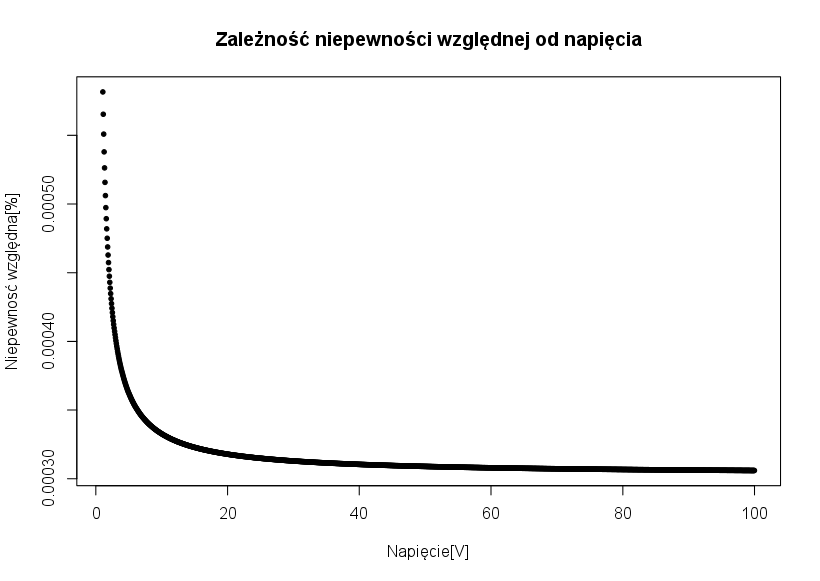
\includegraphics[scale = 0.5]{Wykres2.png}}\\
    \indent Obrazuje to świetnie jak szybko stabilizuje się niepewność względna. Pokazuje to też
    jak niewielkie różnice występują między największą a najmniejszą wartością niepewności
    względnej na całym zakresie pomiarowym.

    \newpage
    \par{Miernik analogowy przejawiał odmienne zachowania. Po pierwsze miernik ten nie pozwala na jakikolwiek pomiar powyżej wybranego zakresu (niektóre mierniki cyfrowe pozwalają na taki pomiar np. Agilent 34401A pozwala na pomiary większe o 20\% zakresu).
    Po drugie pomiary na zakresach o wiele wyższych niż mierzona wartość będą skutkowały brakiem wychylenia wskazówki miernika powyżej zera na skali.
    Widać to przy próbach pomiarów napięcia zasilania 1 V na wyższych zakresach niż zakres 10 V (\textbf{Tabela 5}). Przy próbach pomiaru wskazówka nie wykazała żadnego wychylenia powyżej zera.}\\
    \indent Miernik ten też charakteryzuje się stałą niepewnością bezwzględną dla danego zakresu. Wpływa to negatywnie na niepewność względną, która przyjmuje zachowanie funkcji hiperbolicznej.
    Skutkiem tego jest tym mniejsza niepewność względna im wyższą wartość mierzymy.\\
    \indent Zależność tą przedstawiono na wykresie poniżej. Przedstawia on zmianę niepewności względnej na zakresie 10 V miernika AX-7003 dla wartości od 1 do 10 V:
    \\
    \centerline{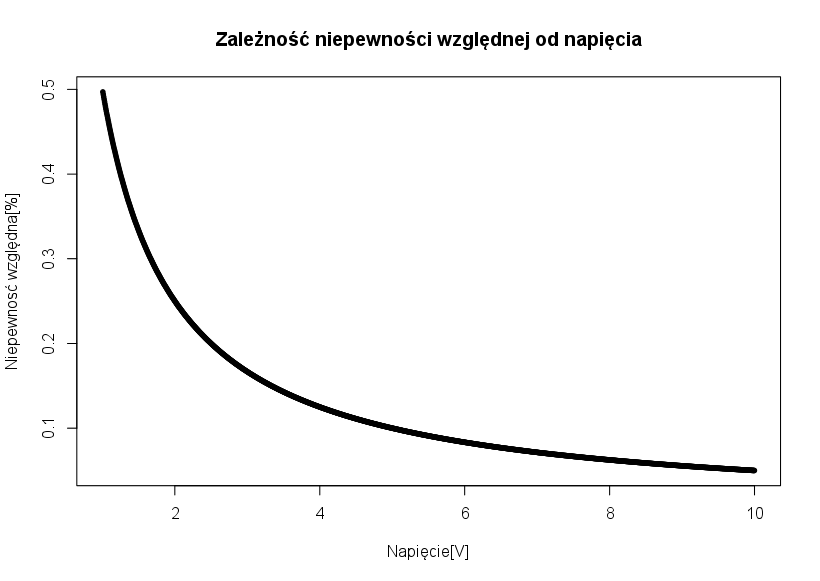
\includegraphics[scale = 0.5]{Wykres1.png}}
    \indent Z powyższego wykresu można wyciągnąć dalsze wnioski, że pomiar miernikiem analogowym powinien odbywać się jak najbliżej wartości maksymalnej zakresu w celu
    uniknięcia dużej niepewności pomiaru.\\

    \tiny{\begin{thebibliography}{9}
         \bibitem{t1}
         https://wzn.pwr.edu.pl/materialy-dydaktyczne/metrologia-elektroniczna
    \end{thebibliography}}
\end{document}
